\documentclass[]{beamer}

\usetheme[numbering=fraction,progressbar=frametitle]{metropolis}

\usepackage[T1]{fontenc}
\usepackage[utf8]{inputenc}
\usepackage[sfdefault,light]{FiraSans}
\usepackage{tikz}
\usepackage{circuitikz}
\usepackage{pgfplots}
\usepackage[spanish]{babel}
\usepackage{booktabs}   % \toprule \midrule \bottomrule
\usepackage{ragged2e}   % \justifying
\usepackage{caption}    % \captionof
\usepackage{subcaption} % subfiguras
\usepackage{graphicx}   % \includegraphics

% Paleta oscuro + verde
\definecolor{darkbg}{HTML}{0A0A0A}
\definecolor{darkgray}{HTML}{1A1A1A}
\definecolor{darkgreen}{HTML}{00CC66}

\setbeamercolor{normal text}{fg=white,bg=darkbg}
\setbeamercolor{frametitle}{fg=darkgreen,bg=darkgray}
\setbeamercolor{progress bar}{fg=darkgreen,bg=darkgray}
\setbeamercolor{alerted text}{fg=darkgreen}
\setbeamercolor{title separator}{fg=darkgreen}
\setbeamercolor{block title}{bg=darkgreen,fg=darkbg}
\setbeamercolor{block body}{bg=darkgray,fg=white}
\setbeamercolor{footline}{bg=darkgray,fg=darkgreen}

\setbeamertemplate{title separator}{\color{darkgreen}\rule{\linewidth}{1.2pt}}

% Pie de página estilo Madrid
\setbeamertemplate{footline}{%
  \leavevmode%
  \hbox{%
  \begin{beamercolorbox}[wd=.33\paperwidth,ht=2.5ex,dp=1ex,leftskip=1em]{footline}%
    \usebeamerfont{author in head/foot}\insertshortauthor
  \end{beamercolorbox}%
  \begin{beamercolorbox}[wd=.34\paperwidth,ht=2.5ex,dp=1ex,center]{footline}%
    \usebeamerfont{title in head/foot}\insertshorttitle
  \end{beamercolorbox}%
  \begin{beamercolorbox}[wd=.33\paperwidth,ht=2.5ex,dp=1ex,rightskip=1em]{footline}%
    \usebeamerfont{date in head/foot}\hfill \insertshortdate \hspace{3em} \insertframenumber{} / \inserttotalframenumber
  \end{beamercolorbox}}%
  \vskip0pt%
}

% Aquí se reactivan los botones estándar de beamer (los de Madrid)
\setbeamertemplate{navigation symbols}{\insertslidenavigationsymbol\insertframenavigationsymbol\insertsubsectionnavigationsymbol\insertsectionnavigationsymbol\insertdocnavigationsymbol\insertbackfindforwardnavigationsymbol}

\setbeamertemplate{frametitle continuation}{}

\title[BJT Base Común]{BJT: Configuración Base Común}
\subtitle{Trabajo Practico N°4}
\author[Grasso, Palombo, Prieto]{%
  \begin{tabular}{l}
      Gaston Grasso -- 401892 \\
    Franco Palombo -- 401910 \\
      Angelo Prieto -- 401012
  \end{tabular}
}
\institute[UTN - FRC]{Universidad Tecnológica Nacional, Facultad Regional Córdoba}
\date[2025]{03/09/2025}
\logo{
\includegraphics[width=.06\textwidth]{images/UTN_logo.png}}

\AtBeginSection[]
{
  \begin{frame}{Tabla de Contenidos}
    \tableofcontents[currentsection]
  \end{frame}
}

\begin{document}

\frame{\titlepage}
\begin{frame}{Tabla de Contenidos}
\tableofcontents
\end{frame}
\chapter{Introducción}

En este trabajo práctico de laboratorio se diseñó un amplificador con transistor BJT en configuración emisor común, utilizando
polarización mediante divisor resistivo bajo el criterio de máxima excursión simétrica (MES). A partir de los cálculos teóricos
se determinaron los valores de las resistencias de polarización y posteriormente se normalizaron a valores comerciales. En ambos
casos se realizaron simulaciones para comprobar que el punto de operación \emph{Q} no se desplazara fuera
de márgenes aceptables, y finalmente se efectuaron mediciones en el laboratorio con las resistencias normalizadas para comparar
los resultados con la simulación.

Además, se llevó a cabo un análisis de pequeña señal. Se calcularon de manera analítica la ganancia de tensión y corriente, así
como las impedancias de entrada y salida del amplificador. Luego, estos parámetros fueron medidos experimentalmente en el laboratorio
con el objetivo de contrastar los resultados teóricos con los prácticos.

\begin{frame}{Introducción}

\begin{figure}
    \centering
    \resizebox{\textwidth}{!}{
    \begin{tikzpicture}
    	% Paths, nodes and wires:
    	\node[npn, rotate=90, yscale=-1] at (-0.02, 2.75){};
    	\draw (2.98, 2.75) to[american resistor, l={$R_C$}] (2.98, 0);
    	\draw (-3.02, 0) to[american resistor, l={$R_1$}] (-0.02, 0);
    	\draw (-3.02, 0) to[american resistor, l={$R_E$}] (-3.02, 2.75);
    	\draw (-0.02, 0) to[american resistor, l={$R_2$}] (2.98, 0);
    	\draw (-0.02, 1.91) -- (-0.02, 0);
    	\draw (-3.02, 2.75) -- (-0.79, 2.75);
    	\draw (0.75, 2.75) -- (2.98, 2.75);
    	\draw (-3.02, 2.75) to[capacitor, l={$C_1$}] (-6.02, 2.75);
    	\draw (5.98, 2.75) to[capacitor, l={$C_C$}] (2.98, 2.75);
    	\draw (5.98, 1.75) to[american resistor, l={$R_L$}] (5.98, -1);
    	\draw (-6.02, 2) to[sinusoidal voltage source, l={$v_i$}] (-6.02, -1);
    	\draw (-0.02, -1.75) to[capacitor, l={$C_2$}] (-0.02, 0);
    	\draw (-3.02, 0) -- (-3.02, -1.75);
    	\draw (-6.02, 2.75) -- (-6.02, 2);
    	\draw (-6.02, -1) -- (-6.02, -1.75) -- (-3.02, -1.75);
    	\draw (2.98, 0) to[battery, l={$V_{CC}$}] (2.98, -1.75);
    	\draw (5.98, -1) |- (2.98, -1.75);
    	\draw (5.98, 1.75) -| (5.98, 2.75);
    	\node[ocirc] at (7.98, 2.75){};
    	\node[ocirc] at (7.98, -1.75){};
    	\draw (5.98, 2.75) -- (7.98, 2.75);
    	\draw (5.98, -1.75) -- (7.98, -1.75);
    	\draw (-3.02, -1.75) -- (2.98, -1.75);
        \node[ground] at (-0.02, -1.75){};
    \end{tikzpicture}
    }
    \caption{circuito amplificador base común.}
\end{figure}
\end{frame}

\section{Características}
\begin{frame}{Características}
\begin{itemize}
    \item Proporciona una alta ganancia de voltaje, pero atenúa la corriente ($A_i \leq 1$).
    \item Tiene baja impedancia de entrada, lo que es útil para ciertas aplicaciones.
    \item Utilizado en: circuitos de radiofrecuencia (RF), amplificadores de banda ancha.
\end{itemize}
\end{frame}

\section{Análisis y diseño}
\begin{frame}{Análisis y diseño}
Para el análisis y/o diseño de un circuito amplificador, se puede hacer uso de la propiedad de superposición.

\only<1>{
\begin{figure}[ht!]
    \centering
    \resizebox{0.5\textwidth}{!}{
        \begin{tikzpicture}
        	% Paths, nodes and wires:
        	\node[npn, rotate=90, yscale=-1](N1) at (-0, 2.75){} node[anchor=south] at (N1.text){$Q_1$};
        	\draw (3, 2.75) to[american resistor, l={$R_C$}] (3, 0);
        	\draw (-3, 0) to[american resistor, l={$R_1$}] (-0, 0);
        	\draw (-3, 0) to[american resistor, l={$R_E$}] (-3, 2.75);
        	\draw (-0, 0) to[american resistor, l={$R_2$}] (3, 0);
        	\draw (-0, 1.91) -- (-0, 0);
        	\draw (-3, 2.75) -- (-0.77, 2.75);
        	\draw (0.77, 2.75) -- (3, 2.75);
        	\draw (-3, 0) -- (-3, -1.75);
        	\draw (0.75, -1.75) to[battery, l={$V_{CC}$}] (-1, -1.75);
        	\draw (-3, -1.75) -- (-1, -1.75);
        	\draw (0.75, -1.75) -| (3, -0);
        \end{tikzpicture}
    }
    \caption{circuito equivalente para CC.}
\end{figure}
}
\only<2>{
\begin{figure}[ht!]
    \centering
    \resizebox{\textwidth}{!}{
        \begin{tikzpicture}
        	% Paths, nodes and wires:
        	\draw (3.25, 1.5) to[american resistor, l={$R_C$}] (3.25, -1.25);
        	\draw (-3.75, -1.25) to[american resistor, l={$R_E$}] (-3.75, 1.5);
        	\draw (5.25, 1.5) to[american resistor, l={$R_L$}] (5.25, -1.25);
        	\draw (-6.23, 1.5) to[sinusoidal voltage source, l={$v_i$}] (-6.25, -1.25);
        	\draw (-1.75, -1.25) to[american resistor, l={$h_{ib}$}] (-1.75, 1.5);
        	\draw (1.25, -1.25) to[american current source, l={$h_{fb} \cdot i_e$}] (1.25, 1.5);
        	\draw (-6.25, -1.25) -- (6.75, -1.25);
        	\node[ocirc] at (6.75, 1.5){};
        	\node[ocirc] at (6.75, -1.25){};
        	\draw (-6.23, 1.5) -| (-1.75, 1.5);
        	\draw (1.25, 1.5) -- (6.75, 1.5);
        \end{tikzpicture}
    }
    \caption{circuito equivalente para CA.}
\end{figure}
}
\end{frame}

\subsection{Polarización}
\begin{frame}{Polarización}
El transistor tiene tres regiones de trabajo: activa, corte y saturación. 
La polarización consiste en definir los componentes de red adecuados, que permitan
que el transistor opere en una región y en un punto determinados. Condición necesaria para
operación en región activa es una polarización emisor-base directa y una polarización
colector-base inversa.
\end{frame}

\subsubsection{Máxima Excursión Simétrica}
\begin{frame}{Máxima Excursión Simétrica}
En particular, se busca ubicar el punto de operación Q en la recta de carga de tal forma que la señal de salida pueda desplazarse con la mayor amplitud
posible antes de alcanzar las regiones de saturación o corte.

Este criterio se conoce como polarización para máxima excursión simétrica (MES).

\begin{figure}[!ht]
  \centering
  \resizebox{0.5\textwidth}{!}{
      \begin{tikzpicture}[x=0.75pt,y=0.75pt,yscale=-1,xscale=1,
                          line cap=round, text=white]
        \definecolor{axis}{HTML}{A0A0A0}
        \definecolor{grid}{HTML}{404040}
        \definecolor{acc1}{HTML}{00CC66}
        \definecolor{acc2}{HTML}{FF6666}
    
        % Ejes
        \draw[axis] (178.6,264.42) -- (472.39,264.42)
                    (194.46,79.16) -- (194.46,278.05)
                    (465.39,259.42) -- (472.39,264.42) -- (465.39,269.42)
                    (189.46,86.16)  -- (194.46,79.16) -- (199.46,86.16);
    
        % Recta verde (acento)
        \draw[acc1, line width=1] (195.14,156.28) -- (435.55,263.48);
    
        % Recta roja
        \draw[acc2, line width=1] (194.45,133.48) -- (379.39,262.94);
    
        % Punto Q negro -> blanco
        \draw[fill=white, draw=white] (283.94,198.21)
          circle [x radius=2.98, y radius=2.98];
    
        % Curva izquierda
        \draw[axis] (101.24,198.21) .. controls (108.78,165.05) and (115.99,133.48) ..
          (124.35,133.48) .. controls (132.72,133.48) and (139.93,165.05) ..
          (147.47,198.21) .. controls (155.01,231.37) and (162.22,262.94) ..
          (170.59,262.94) .. controls (178.96,262.94) and (186.17,231.37) ..
          (193.71,198.21) .. controls (193.95,197.13) and (194.2,196.04) ..
          (194.45,194.96);
    
        % Guías punteadas
        \draw[grid, dash pattern={on 4.5pt off 4.5pt}]
          (101.98,133.48) -- (194.45,133.48)
          (101.99,264.42) -- (194.46,264.42)
          (101.98,198.21) -- (286.92,198.21)
          (286.92,198.21) -- (286.51,358.87)
          (379.39,262.94) -- (379.39,355.41)
          (194.45,262.94) -- (194.45,355.41);
    
        % Onda derecha
        \draw[axis] (286.88,266.02) .. controls (334.25,273.53) and (379.35,280.72) ..
          (379.35,289.09) .. controls (379.36,297.46) and (334.27,304.69) ..
          (286.91,312.26) .. controls (239.54,319.82) and (194.45,327.06) ..
          (194.46,335.42) .. controls (194.46,343.79) and (239.56,350.98) ..
          (286.93,358.49) .. controls (287.09,358.52) and (287.25,358.54) ..
          (287.42,358.57);
    
        % Flechas
        \draw[axis] (286.92,133.48) -- (251.34,169.06);
        \draw[axis, shift={(249.93,170.47)}, rotate=315] (6.56,-1.97) --
          (0,0) -- (6.56,1.97);
        \draw[axis] (434.87,207.46) -- (399.3,243.03);
        \draw[axis, shift={(397.88,244.45)}, rotate=315] (6.56,-1.97) --
          (0,0) -- (6.56,1.97);
    
        % Textos
        \draw (292.24,275.1) node[font=\tiny] {$\displaystyle V_{CEQ}$};
        \draw (172.55,182.55) node[font=\tiny] {$\displaystyle I_{CQ}$};
        \draw (202.71,79.9)   node[font=\tiny] {$\displaystyle I_{C}$};
        \draw (473.73,254.25) node[font=\tiny] {$\displaystyle V_{CB}$};
        \draw (287.64,119.68) node[font=\scriptsize] {$\displaystyle m_{ca}$};
        \draw (432.14,192.26) node[font=\scriptsize] {$\displaystyle m_{cc}$};
        \draw (383.71,272.76) node[font=\tiny] {$\displaystyle 2V_{CEQ}$};
        \draw (166.67,117.46) node[font=\tiny] {$\displaystyle 2I_{CQ}$};
        \draw (285.64,180.08) node[font=\scriptsize] {$\displaystyle Q_{MES}$};
      \end{tikzpicture}
    }
  \caption{gráfica punto $Q_{MES}$.}
  \label{fig:gráfica-mes}
\end{figure}
\end{frame}

\begin{frame}[allowframebreaks]{Malla de salida}
\begin{figure}[H]
    \centering
    \begin{minipage}{0.4\textwidth}
        \centering
        \resizebox{0.6\textwidth}{!}{
        \begin{tikzpicture}
            \node[npn](N1) at (1.59, 2){} node[anchor=west] at (N1.text){$Q1$};
            \draw (1.59, 1.25) to[american resistor, l={$R_E$}] (1.59, -1);
            \draw (1.59, 5.02) to[american resistor, l={$R_c$}] (1.59, 2.77);
            \draw (1.59, -1) -| (1.59, -1.25);
            \node[vcc](N2) at (1.59, 6){} node[anchor=south] at (N2.text){$V_{cc}$};
            \draw (1.59, 5.25) -| (1.59, 6);
            \node[ground] at (1.59, -1.75){};
            \draw (1.59, -1.25) -| (1.59, -1.75);
            \draw (-1.66, 2) to[american resistor, l={$R_B$}] (-1.66, -0.25);
            \draw (-1.66, -0.25) to[battery1, l={$V_{BB}$}] (-1.66, -1.5);
            \draw (-1.66, 2) -| (0.75, 2);
            \draw (-1.66, -1.5) -| (-1.66, -1.75) -- (1.59, -1.75);
            \draw (1.59, 5.02) -| (1.59, 5.25);
        \end{tikzpicture}
    }
        \caption{Circuito para CC simplificado por Thévenin.}
        \label{fig:malla-salida}
    \end{minipage}%
    \begin{minipage}{0.45\textwidth}
        \centering
        Donde $R_{B}$ es la resistencia equivalente y $V_{BB}$ es la tensión de Thévenin:
        \begin{align}
            R_{B} &= R_1||R_2=\frac{R_1 R_2}{R_1 + R_2} \label{ec:thevenin-rb}\\[6pt]
            V_{BB} &= V_{CC} \cdot \frac{R_1}{R_1 + R_2} \label{ec:thevenin-vbb}
        \end{align}
        Se debe determinar los valores de $R_B$ y $V_{BB}$ con el objetivo de polarizar
        el transistor para MES.
    \end{minipage}
\end{figure}

Aplicando LKV a la malla de salida:

\begin{align}
    V_{CC} - I_{CQ}R_C - V_{CBQ} - \frac{I_{CQ}}{\beta}R_B - V_{BB} &= 0 \label{ec:malla-salida-cc}
\end{align}

\begin{figure}[!ht]
  \centering
  \begin{minipage}{0.45\textwidth}
  \resizebox{0.6\textwidth}{!}{
    \begin{tikzpicture}
    	% Paths, nodes and wires:
    	\node[npn, rotate=90, yscale=-1] at (-0, 1.5){};
    	\draw (2, 1.5) to[american resistor, l={$R_C$}] (2, -1.25);
    	\draw (4, 1.5) to[american resistor, l={$R_L$}] (4, -1.25);
    	\draw (-0, 0.66) -- (-0, -1.25) -- (4, -1.25);
    	\draw (0.75, 1.5) -- (4, 1.5);
    	\node[ground] at (-0, -1.25){};
    \end{tikzpicture}
    }
    \caption{malla de salida para $CA$.}
    \label{fig:malla-salida-ca}
  \end{minipage}
  \begin{minipage}{0.45\textwidth}
    \centering
    LKV:
    \begin{align}
        \hat{v}_{cb} &= \hat{\imath}_c(R_C ||R_L) \nonumber \\[6pt]
        \hat{v}_{cb} &= \hat{\imath}_c\frac{R_C R_L}{R_C + R_L} \nonumber \\[6pt]
        \hat{v}_{cb} &= \hat{\imath}_c(R_{CA}) \label{ec:malla-salida-ca}
    \end{align}
  \end{minipage}
\end{figure}

Por definición de MES, se tiene que la amplitud pico de la señal de salida es:
\begin{align*}
    \hat{v}_{cb} &= V_{CBQ}\\[6pt]
    \hat{\imath}_c &= I_{CQ}
\end{align*}

Reemplazando esto en la ecuación \ref{ec:malla-salida-ca}:

\begin{align*}
    V_{CBQ} &= I_{CQ}(R_{CA})
\end{align*}

Y reemplazando esta última igualdad en la ecuación \ref{ec:malla-salida-cc}:

\begin{align}
    V_{CC} - I_{CQ}R_C - V_{CBQ} + \frac{I_{CQ}}{\beta}R_B - V_{BB} &= 0 \nonumber \\[6pt]
    V_{CC} - I_{CQ}R_C - I_{CQ}(R_{CA}) + \frac{I_{CQ}}{\beta}R_B - V_{BB} &= 0 \nonumber \\[6pt]
    I_{CQ} = \frac{V_{CC} - V_{BB}}{R_C-\frac{R_B}{\beta} + (R_{CA})} \\[6pt]
    I_{CQ_{MES}} = \frac{V_{CC} - V_{BB}}{(R_{CC}) + (R_{CA})} \label{ec:iq-mes}
\end{align}

\begin{minipage}[][\textheight][]{\textwidth}
Despejando para $V_{CB}$:
\begin{align}
    V_{CC} - I_{CQ}R_C - V_{CBQ} + \frac{I_{CQ}}{\beta}R_B - V_{BB} &= 0 \nonumber \\[6pt]
    V_{CBQ_{MES}} = V_{CC} - V_{BB} - I_{CQ_{MES}}(R_{CC})
\end{align}
\end{minipage}

\end{frame}

\begin{frame}[allowframebreaks]{Determinación de $V_{BB}$ y $R_B$}
Para determinar $V_{BB}$ se tiene que aplicar LKV a la malla de entrada.

\begin{figure}[H]
    \centering
    \begin{minipage}{0.4\textwidth}
        \centering
        \resizebox{0.6\textwidth}{!}{
            \begin{tikzpicture}
              % Paths, nodes and wires:
              \node[npn](N1) at (0, 0){} node[anchor=west] at (N1.text){$Q1$};
              \draw (0, -0.77) to[american resistor, l={$R_E$}] (0, -3);
              \draw (0, 3.02) to[american resistor, l={$RC$}] (0, 0.77);
              \draw (0, -3) -| (0, -3.25);
              \node[vcc](N2) at (0, 3.02){} node[anchor=south] at (N2.text){$V{cc}$};
              \node[ground] at (0, -3.75){};
              \draw (0, -3.25) -| (0, -3.75);
              \draw (-3.25, 0) to[american resistor, l={$RB$}] (-3.25, -2.25);
              \draw (-3.25, 0) -- (-0.84, 0);
              \draw (-3.25, -3.5) -| (-3.25, -3.75) -- (0, -3.75);
              \draw (-3.25, -2.25) to[battery, l={$V{BB}$}] (-3.25, -3.5);
            \end{tikzpicture}
    }
        \caption{Circuito para CC simplificado por Thévenin.}
        \label{fig:malla-entrada}
    \end{minipage}%
    \begin{minipage}{0.4\textwidth}
        \centering
        LKV:
        \begin{align}
            V_{BB} - I_{BQ}R_B - V_{BE}-I_{EQ}R_E &= 0 \nonumber\\[6pt]
            V_{BB} - \frac{I_{CQ}}{\beta}R_B - V_{BE}-I_{CQ}R_E &= 0 \nonumber\\[6pt]
            I_{CQ} = \frac{V_{BB} - V_{BE}}{\frac{R_B}{\beta}+R_E}
        \end{align}
    \end{minipage}
\end{figure}

Igualando esta ecuación con la ecuación de $I_{CQ_{MES}}$ (Ec. \ref{ec:iq-mes}):

\begin{gather*}
    \frac{V_{CC}-V_{BB}}{R_{CC} + R_{CA}}= \frac{V_{BB}-V_{BE}}{\frac{R_B}{\beta}+R_E} \nonumber\\[6pt]
    V_{CC}(\frac{R_B}{\beta}+R_E) - V_{BB}(\frac{R_B}{\beta}+R_E) = V_{BB}(R_{CC}+R_{CA}) - V_{BE}(R_{CC}+R_{CA}) \nonumber\\[6pt]
    V_{BB} = \frac{V_{CC}(\frac{R_B}{\beta}+R_E) + V_{BE}(R_{CC}+R_{CA})}{\frac{R_B}{\beta}+R_E + R_{CC} + R_{CA}} \nonumber\\[6pt]
    V_{BB} = \frac{V_{CC}(\frac{R_B}{\beta}+R_E) + V_{BE}(R_C-\frac{R_B}{\beta}+R_C||R_L)}{R_E + R_C + R_C||R_L}\\[6pt]
\end{gather*}

$R_B$ se puede determinar considerando el siguiente criterio de diseño:

\begin{equation}
    R_E  \gg \frac{R_b}{\beta} \therefore R_E = 10\frac{R_B}{\beta} \therefore \frac{R_B}{\beta} = \frac{R_E}{10} \label{ec:criterio-diseño}
\end{equation}

Finalmente, para determinar el valor de $R_1$ y $R_2$, se consideran las ecuaciones (\ref{ec:thevenin-rb}) y (\ref{ec:thevenin-vbb}), resultantes de aplicar Thévenin a la malla de entrada del circuito 
amplificador, y la ecuación \ref{ec:criterio-diseño},
resultante de establecer el criterio de diseño:

\begin{align*}
    R_B &= R_1||R_2=\frac{R_1 R_2}{R_1 + R_2} \tag{\ref{ec:thevenin-rb}}\\[6pt]
    V_{BB} &= V_{CC} \cdot \frac{R_1}{R_1 + R_2} \tag{\ref{ec:thevenin-vbb}}\\[6pt]
    R_B &= \boxed{\beta \frac{R_E}{10}} \tag{\ref{ec:criterio-diseño}}
\end{align*}

Ahora que los valores de $R_B$ y $V_{BB}$ se pueden determinar, se puede proceder a 
despejar $R_1$ y  $R_2$ de las ecuaciones correspondientes, obteniendo:

\begin{center}
    \begin{minipage}{0.3\textwidth}
    \begin{equation*}
        \boxed{R_1 = \frac{R_B}{1-\frac{V_{BB}}{V_{CC}}}}
    \end{equation*}
    \end{minipage}
    \begin{minipage}{0.3\textwidth}
    \begin{equation*}
        \boxed{R_2 = \frac{V_{CC}R_B}{V_{BB}}}
    \end{equation*}
    \end{minipage}
\end{center}
\end{frame}

\subsection{Pequeña señal}
\begin{frame}[allowframebreaks]{Análisis para pequeñal señal}
Para el análisis de pequeña señal, se considera un circuito equivalente del transistor en
base común.

\begin{figure}
    \centering
    \resizebox{0.8\textwidth}{!}{
    \begin{tikzpicture}
    	% Paths, nodes and wires:
    	\draw (3.625, 1.25) to[american resistor, l={$\frac{1}{h_{ob}}$}] (3.625, -1.5);
    	\draw (-4.375, 1.25) to[american resistor, l={$h_{ib}$}] (-2.625, 1.25);
    	\draw (1.75, -1.5) to[american current source, l={$h_{fb} \cdot i_e$}] (1.75, 1.25);
    	\draw (-1.25, 1.25) to[american voltage source, l_={$h_{rb}V_{CB}$}] (-1.25, -1.5);
    	\draw (-2.625, 1.25) -| (-1.25, 1.25);
    	\draw (1.75, 1.25) -- (5.5, 1.25);
    	\draw (-4.375, 1.25) -| (-5.25, 1.25);
    	\draw (5.375, -1.5) -- (-5.25, -1.5);
    	\node[shape=rectangle, draw, line width=1pt, minimum width=9.215cm, minimum height=4.465cm] at (0.125, -0){};
    	\node[ground] at (0.25, -1.5){};
    	\node[shape=rectangle, minimum width=0.465cm, minimum height=0.59cm] at (0.25, -1.188){} node[anchor=north west, align=left, text width=0.077cm, inner sep=6pt] at (0, -0.875){B};
    	\node[shape=rectangle, minimum width=0.465cm, minimum height=0.59cm] at (5.25, 1.562){} node[anchor=north west, align=left, text width=0.077cm, inner sep=6pt] at (5, 1.875){C};
    	\node[shape=rectangle, minimum width=0.465cm, minimum height=0.59cm] at (-5, 1.562){} node[anchor=north west, align=left, text width=0.077cm, inner sep=6pt] at (-5.25, 1.875){E};
    	\node[ocirc] at (5.5, 1.25){};
    	\node[ocirc] at (5.375, -1.5){};
    	\node[ocirc] at (-5.25, 1.25){};
    	\node[ocirc] at (-5.25, -1.5){};
    	\draw[-latex] (4.5, 1.5) -- (3.75, 1.5);
    	\draw[-latex] (-1, 1) |- (-1.5, 1.5);
    \end{tikzpicture}
    }
    \caption{circuito equivalente para pequeña señal de transitor en base común.}
\end{figure}

$h_{rb}$ y $h_{ob}$ despreciables.
\begin{figure}[ht!]
    \centering
    \resizebox{\textwidth}{!}{
        \begin{tikzpicture}
        	% Paths, nodes and wires:
        	\draw (3.25, 1.5) to[american resistor, l={$R_C$}] (3.25, -1.25);
        	\draw (-3.75, -1.25) to[american resistor, l={$R_E$}] (-3.75, 1.5);
        	\draw (5.25, 1.5) to[american resistor, l={$R_L$}] (5.25, -1.25);
        	\draw (-6.23, 1.5) to[sinusoidal voltage source, l={$v_i$}] (-6.25, -1.25);
        	\draw (-1.75, -1.25) to[american resistor, l={$h_{ib}$}] (-1.75, 1.5);
        	\draw (1.25, -1.25) to[american current source, l={$h_{fb} \cdot i_e$}] (1.25, 1.5);
        	\draw (-6.25, -1.25) -- (6.75, -1.25);
        	\node[ocirc] at (6.75, 1.5){};
        	\node[ocirc] at (6.75, -1.25){};
        	\draw (-6.23, 1.5) -| (-1.75, 1.5);
        	\draw (1.25, 1.5) -- (6.75, 1.5);
        \end{tikzpicture}
    }
    \caption{circuito equivalente para CA.}
\end{figure}
\end{frame}

\begin{align*}
    h_{ib} &= \frac{v_{eb}}{-i_e} = \frac{-v_{be}}{-i_e} = \frac{i_b h_{ie}}{i_b(h_{fe}+1)}=\frac{h_{ie}}{h_{fe}+1}\\[6pt]
    h_{fb} &= \frac{i_c}{-i_e} = \frac{i_{b}h_{fe}}{-i_b({h_{fe}+1})} \approx -1
\end{align*}

\section{Diseño}
\begin{frame}{Circuitos equivalentes}
  \begin{minipage}[t]{0.45\textwidth}
    \resizebox{\textwidth}{!}{
      \begin{tikzpicture}
      % Paths, nodes and wires:
      \node[npn, rotate=90, yscale=-1](N1) at (0, -0){} node[anchor=south] at (N1.text){$Q_1$};
      \draw (-0.77, 0) |- (-3, -0);
      \draw (0.77, -0) -- (3, -0);
      \draw (-3, -0.84) to[american resistor, l={$R_E$}] (-3, -2.75);
      \draw (3, -0.84) to[american resistor, l={$R_C$}] (3, -2.75);
      \draw (-3, -0.84) -| (-3, -0);
      \draw (3, -0) -| (3, -0.84);
      \node[vcc](N2) at (5, -3){} node[anchor=south] at (N2.text){$V_{CC}$};
      \draw (5, -3) -| (5, -4) -- (3, -4);
      \draw (-3, -2.75) |- (-3, -4);
      \draw (3, -2.75) -| (3, -4);
      \node[ground] at (-3, -4){};
      \draw (-3, -0) -- (-4, -0);
      \draw (3, -0) -- (6, -0);
      \node[ocirc](N3) at (-4, -0){} node[anchor=east] at (N3.text){$V_i$};
      \node[ocirc](N4) at (6, -0){} node[anchor=west] at (N4.text){$V_o$};
      \draw (-2.41, -3.5) to[american resistor, l={$R_1$}] (-0.5, -3.5);
      \draw (0.5, -3.5) to[american resistor, l={$R_2$}] (2.41, -3.5);
      \draw (-2.41, -3.5) -- (-3, -3.5);
      \draw (-0.5, -3.5) -- (0.5, -3.5);
      \draw (2.41, -3.5) -- (3, -3.5);
      \draw (0, -3.5) |- (-0, -0.84);
    \end{tikzpicture}
    }
    Según (Ec. \ref{eq:r1}) y (Ec. \ref{eq:r2}) tenemos que:
    \begin{equation*}
      R_1 = \frac{R_B}{1 - \frac{V_{BB}}{V_{CC}}} \quad R_2 = \frac{V_{CC} R_B}{V_{BB}}
    \end{equation*}
  \end{minipage}
  \begin{minipage}{0.08\textwidth}
    \begin{equation*}
      \equiv
    \end{equation*}
  \end{minipage}
  \begin{minipage}[t]{0.45\textwidth}
    \resizebox{\textwidth}{!}{
    \begin{tikzpicture}
      % Paths, nodes and wires:
      \node[npn, rotate=90, yscale=-1](N1) at (0, -0){} node[anchor=south] at (N1.text){$Q_1$};
      \draw (-0, -0.84) to[american resistor, l={$R_B$}] (0, -2.75);
      \draw (-0.77, 0) |- (-3, -0);
      \draw (0.77, -0) -- (3, -0);
      \draw (-3, -0.84) to[american resistor, l={$R_E$}] (-3, -2.75);
      \draw (3, -0.84) to[american resistor, l={$R_C$}] (3, -2.75);
      \draw (0, -2.75) to[battery, l={$V_{BB}$}] (0, -4);
      \draw (-3, -0.84) -| (-3, -0);
      \draw (3, -0) -| (3, -0.84);
      \node[vcc](N2) at (5, -3){} node[anchor=south] at (N2.text){$V_{CC}$};
      \draw (5, -3) -| (5, -4) -- (3, -4);
      \draw (-3, -2.75) |- (0, -4);
      \draw (3, -2.75) -| (3, -4);
      \node[ground] at (0, -4){};
      \draw (-3, -0) -- (-4, -0);
      \draw (3, -0) -- (6, -0);
      \node[ocirc](N3) at (-4, -0){} node[anchor=east] at (N3.text){$V_i$};
      \node[ocirc](N4) at (6, -0){} node[anchor=west] at (N4.text){$V_o$};
    \end{tikzpicture}
    }
    Según (Ec. \ref{ec:thevenin-rb}) y (Ec. \ref{ec:thevenin-vbb}) tenemos que:
    \begin{equation*}
      R_B = \frac{R_1 R_2}{R_1 + R_2} \quad V_{BB} = \frac{V_{CC} R_1}{R_1 + R_2}
    \end{equation*}
  \end{minipage}
\end{frame}
\subsection{Punto Q}
\begin{frame}[allowframebreaks]{Polarización en CC}
  \begin{minipage}{0.3\textwidth}
    \resizebox{\textwidth}{!}{
    \begin{tikzpicture}
      % Paths, nodes and wires:
      \node[npn](N1) at (0, 0){} node[anchor=west] at (N1.text){$Q1$};
      \draw (0, -0.77) to[american resistor, l={$R_E$}] (0, -3);
      \draw (0, 3.02) to[american resistor, l={$R_C$}] (0, 0.77);
      \draw (0, -3) -| (0, -3.25);
      \node[vcc](N2) at (0, 3.02){} node[anchor=south] at (N2.text){$V_{cc}$};
      \node[ground] at (0, -3.75){};
      \draw (0, -3.25) -| (0, -3.75);
      \draw (-3.25, 0) to[american resistor, l={$R_B$}] (-3.25, -2.25);
      \draw (-3.25, 0) -- (-0.84, 0);
      \draw (-3.25, -3.5) -| (-3.25, -3.75) -- (0, -3.75);
      \draw (-3.25, -2.25) to[battery, l={$V_{BB}$}] (-3.25, -3.5);
      \draw (0, 0.77) -- (1, 0.77);
      \draw (0, -0.77) -- (1, -0.77);
      \node[ocirc](N3) at (1, -0.77){} node[anchor=west] at (N3.text){$V_i$};
      \node[ocirc](N4) at (1, 0.77){} node[anchor=west] at (N4.text){$V_o$};
    \end{tikzpicture}
    }
    \begin{align*}
      V_{CC} &= 15.2V \quad R_E = 220\Omega\\
      R_C &= 2K2\Omega \quad \beta = 484\\
      &\quad \quad R_L = 2K2\Omega
    \end{align*}
  \end{minipage}
  \begin{minipage}{0.6\textwidth}
    Aplicando el criterio de diseño:
    \begin{equation}
      R_B = R_E \frac{\beta}{10}
    \end{equation}
    Se obtiene:
    \begin{align*}
      R_B &= 2K2\Omega \frac{484}{10}\\[6pt]
      R_B &= 10648 \Omega
    \end{align*}
  \end{minipage}
  \begin{minipage}[][\textheight][]{\textwidth}
    Usando (Ec. \ref{ec:vbb}):
    \small
    \begin{align*}
      V_{BB} &= \frac{V_{CC} \left(R_E + \frac{R_B}{\beta}\right) + V_{BE} \left(R_C - \frac{R_B}{\beta} + R_C // R_L \right)}{R_E + R_C + R_C // R_L}\\[6pt]
      V_{BB} &= \frac{15.2V \left(220\Omega + \frac{10684\Omega}{484}\right) + 0.7V \left(2K2\Omega - \frac{10684\Omega}{484} + 2K2\Omega // 2K2\Omega \right)}{220\Omega + 2K2\Omega + 2K2\Omega // 2K2\Omega}\\[6pt]
      V_{BB} &= 1.69V
    \end{align*}
  \end{minipage}

  Procedemos a calcular $R_1$ y $R_2$ usando (Ec. \ref{eq:r1}) y (Ec. \ref{eq:r2}):
  \begin{figure}[!ht]
    \begin{minipage}{0.45\textwidth}
      \begin{align*}
        R_2 &= \frac{V_{CC} R_B}{V_{BB}}\\[6pt]
        R_2 &= \frac{15.2V \cdot 10648\Omega}{1.69V}\\[6pt]
        R_2 &= 95768.99\Omega
      \end{align*}
    \end{minipage}
    \hfill
    \begin{minipage}{0.45\textwidth}
      \begin{align*}
        R_1 &= \frac{R_B R_2}{R_2 - R_B}\\[6pt]
        R_1 &= \frac{95768.99\Omega \cdot 10648\Omega}{95768.99\Omega - 10648\Omega}\\[6pt]
        R_1 &= 11979.98\Omega
      \end{align*}
    \end{minipage}
  \end{figure}
  \begin{figure}[!ht]
    Por ultimo, calculamos $I_{CQ_{MES}}$ y $V_{CBQ_{MES}}$ usando (Ec. \ref{ec:iq-mes}) y (Ec. \ref{ec:vcb-mes}):
    \small
    \begin{minipage}{0.45\textwidth}
      \begin{align*}
        I_{CQ_{MES}} &= \frac{V_{CC} - V_{BB}}{R_C - \frac{R_B}{\beta} + R_C // R_L}\\[6pt]
        I_{CQ_{MES}} &= \frac{15.2V - 1.69V}{2K2\Omega - \frac{10648\Omega}{484} + 2K2\Omega // 2K2\Omega}\\[6pt]
        I_{CQ_{MES}} &= 4.121mA
      \end{align*}
    \end{minipage}
    \hfill
    \begin{minipage}{0.45\textwidth}
      \begin{align*}
        V_{CBQ_{MES}} &= V_{CC} - V_{BB} - I_{CQ_{MES}} \left(R_C - \frac{R_B}{\beta}\right)\\[6pt]
        V_{CBQ_{MES}} &= 15.2V - 1.69V - 4.121mA \left(2K2\Omega - \frac{10648\Omega}{484}\right)\\[6pt]
        V_{CBQ_{MES}} &= 4.53V
      \end{align*}
    \end{minipage}
  \end{figure}
\end{frame}

\begin{frame}[allowframebreaks]{Rectas de Carga}
  \begin{figure}[!h]
    \begin{minipage}[t]{0.45\textwidth}
      Recta de carga en CC:
      \begin{equation*}
        v_{CBQ} = V_{CC} - V_{BB} - i_C \left(R_C - \frac{R_B}{\beta}\right)
      \end{equation*}
    \end{minipage}
    \hfill
    \begin{minipage}[t]{0.45\textwidth}
      Recta de carga en CA:
      \begin{align*}
        v_{CB} &= V_{CC}' - i_C \frac{R_C R_L}{R_C + R_L}\\[6pt]
        V_{CC}' &= V_{CBQ_{MES}} + I_{CQ_{MES}}(R_C // R_L)
      \end{align*}
    \end{minipage}
  \end{figure}
  Los cortes en los ejes están dados por:
  \begin{figure}[!ht]
    \begin{minipage}{0.45\textwidth}
      Para CC:
      \small
      \begin{align*}
        &i_C \to 0, \quad v_{CB_{max}} = V_{CC} - V_{BB}\\[6pt]
        &v_{CB} \to 0, \quad i_{C_{max}} = \frac{V_{CC} - V_{BB}}{R_C - \frac{R_B}{\beta}}
      \end{align*}
    \end{minipage}
    \hfill
    \begin{minipage}{0.45\textwidth}
      Para CA:
      \small
      \begin{align*}
        &i_C \to 0, \quad v_{CB_{max}} = V_{CC}'\\[6pt]
        &v_{CB} \to 0, \quad i_{C_{max}} = \frac{V_{CBQ_{MES}}}{R_C // R_L} + I_{CQ_{MES}}
      \end{align*}
    \end{minipage}
  \end{figure}

  \begin{figure}[!h]
    \centering
    \begin{minipage}{0.45\textwidth}
      \centering
      \begin{tikzpicture}
        \begin{axis}[
            axis lines=middle,
            xlabel={$V_{CB}$ [V]},
            ylabel={$I_C$ [mA]},
            xmin=0, xmax=16,
            ymin=0, ymax=10,
            grid=both,
            width=6cm,
            height=6cm,
            xtick={0,2,...,15},
            ytick={0,2,...,7},
            legend style={fill=darkbg, draw=white},
        ]
          \addplot[red, thick] coordinates {(0,6.2) (13.51,0)};
          \addlegendentry{Recta CC}
          \addplot[blue, thick] coordinates {(0,8.23) (9.06,0)};
          \addlegendentry{Recta CA}
          \addplot[only marks, mark=*] coordinates {(4.525,4.125)};
          \node[above right] at (axis cs:4.525,4.125) {Q};
        \end{axis}
      \end{tikzpicture}
    \end{minipage}
    \hfill
    \begin{minipage}{0.45\textwidth}
      \begin{gather*}
        v_{CBQ_{CC}} = v_{CB_{CA}}\\[6pt]
        i_C = \frac{V_{CC} - V_{BB} - V_{CC}'}{R_C - \frac{R_B}{\beta} - R_C // R_L}\\[6pt]
        i_C = 4.125mA \to v_{CBQ} = 4.525V
      \end{gather*}
    \end{minipage}
    \caption{rectas de carga y punto Q extraído de las intersecciones de las rectas.}
  \end{figure}

\end{frame}

\begin{frame}{Simulación}
  \begin{figure}[!ht]
    \centering
    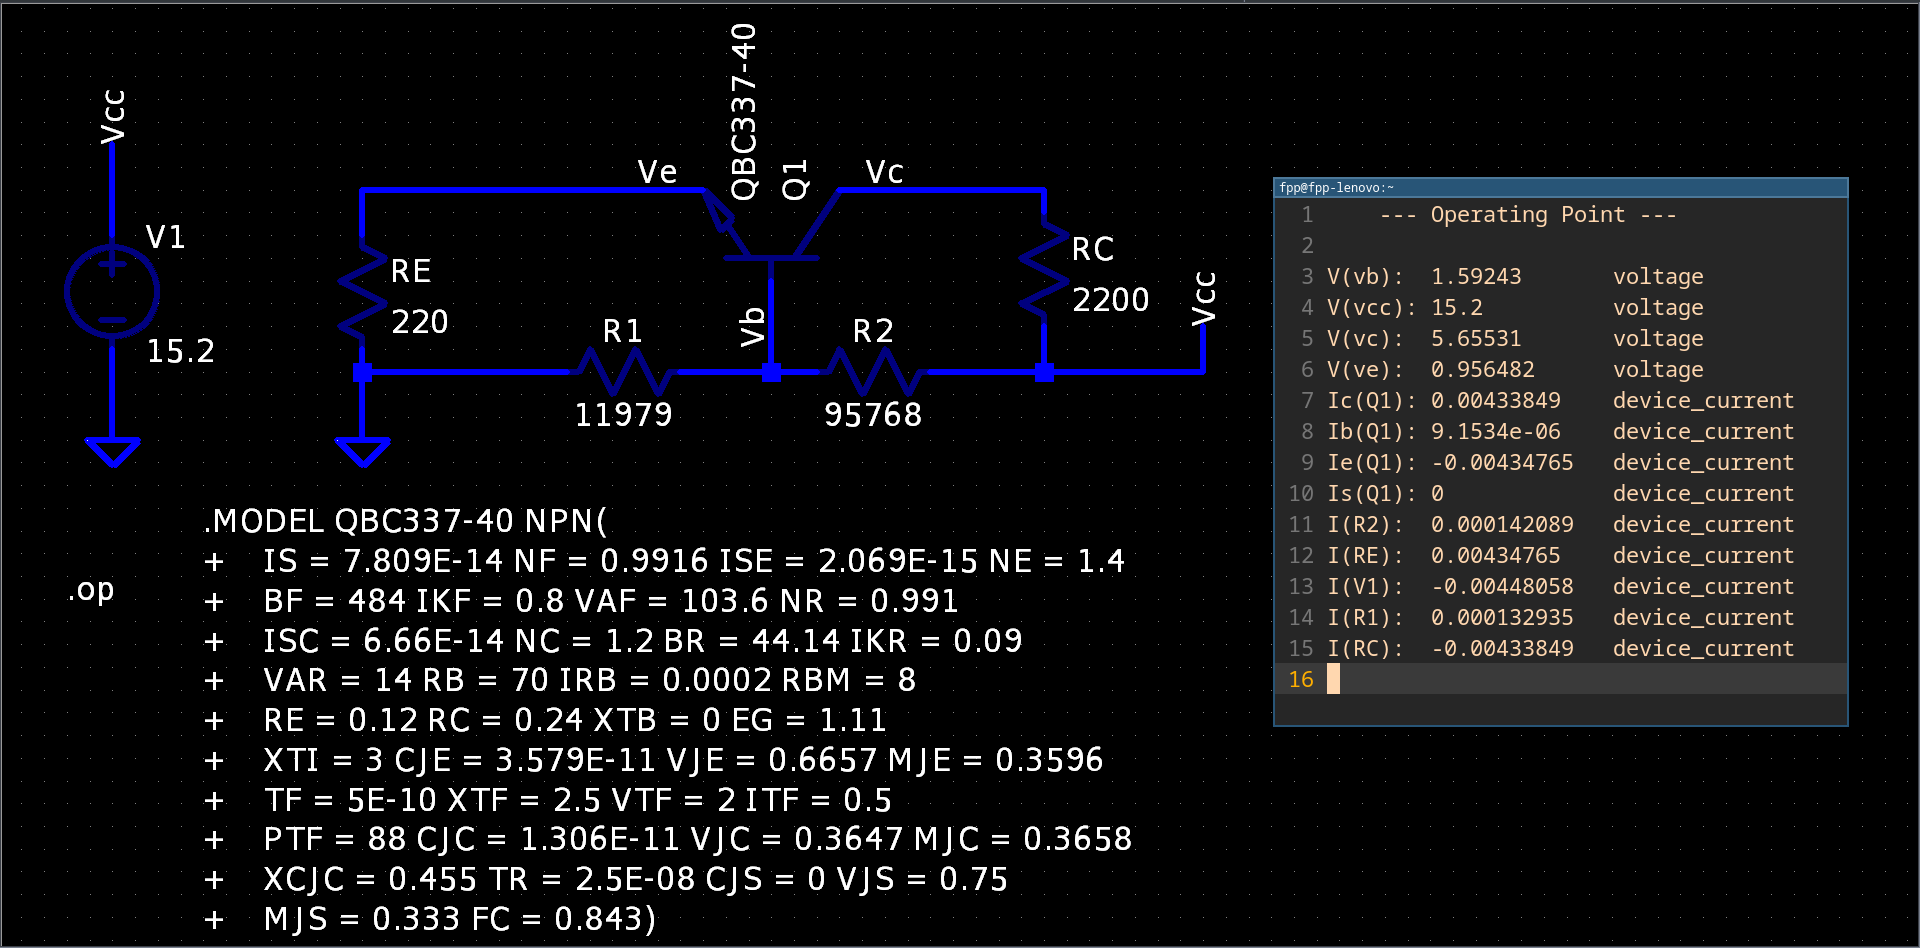
\includegraphics[width=.9\textwidth]{images/sim_calculada.png}
    \caption{simulación en LTSpice de punto de operación (OP).}
  \end{figure}
  \begin{equation*}
    4.07V \leq v_{CBQ} \leq 4.98V \quad \quad 3.7mA \leq i_{CQ} \leq 4.53mA
  \end{equation*}
\end{frame}

\subsection{Normalización}
\begin{frame}[allowframebreaks]{Normalización de Resistores}
  Los valores comerciales mas cercanos a los valores calculados de $R_1$ y $R_2$ son:
  \begin{block}{Valores Normalizados}
    \begin{equation*}
      R_1 = 11979\Omega \to R_1 = 12K\Omega \quad R_2 = 95768\Omega \to R_2 = 100K\Omega
    \end{equation*}
  \end{block}
  Es necesario volver a calcular el punto Q para corroborar que este dentro del 10\% de margen permitido.

  Usando (Ec. \ref{ec:thevenin-rb}) y (Ec. \ref{ec:thevenin-vbb}):
  \begin{figure}[!ht]
    \begin{minipage}{0.45\textwidth}
      \begin{align*}
        R_B &= \frac{R_1 R_2}{R_1 + R_2}\\[6pt]
        R_B &= \frac{12K\Omega \cdot 100K\Omega}{12K\Omega + 100K\Omega}\\[6pt]
        R_B &= 10714\Omega
      \end{align*}
    \end{minipage}
    \hfill
    \begin{minipage}{0.45\textwidth}
      \begin{align*}
        V_{BB} &= \frac{V_{CC} R_1}{R_1 + R_2}\\[6pt]
        V_{BB} &= \frac{15.2V \cdot 12K\Omega}{12K\Omega + 100K\Omega}\\[6pt]
        V_{BB} &= 1.62V
      \end{align*}
    \end{minipage}
  \end{figure}
  \begin{figure}[!ht]
    Podemos calcular nuevamente $I_{CQ}$ y $V_{CBQ}$ usando (Ec. \ref{ec:iq-mes}) y (Ec. \ref{ec:vcb-mes}):
    \small
    \begin{minipage}{0.45\textwidth}
      \begin{align*}
        I_{CQ_{MES}} &= \frac{V_{CC} - V_{BB}}{R_C - \frac{R_B}{\beta} + R_C // R_L}\\[6pt]
        I_{CQ_{MES}} &= \frac{15.2V - 1.62V}{2K2\Omega - \frac{10714\Omega}{484} + 2K2\Omega // 2K2\Omega}\\[6pt]
        I_{CQ_{MES}} &= 4.142mA
      \end{align*}
    \end{minipage}
    \hfill
    \begin{minipage}{0.45\textwidth}
      \begin{align*}
        V_{CBQ_{MES}} &= V_{CC} - V_{BB} - I_{CQ_{MES}} \left(R_C - \frac{R_B}{\beta}\right)\\[6pt]
        V_{CBQ_{MES}} &= 15.2V - 1.62V - 4.142mA \left(2K2\Omega - \frac{10714\Omega}{484}\right)\\[6pt]
        V_{CBQ_{MES}} &= 4.55V
      \end{align*}
    \end{minipage}
  \end{figure}

  Los valores de polarización calculados con las resistencias normalizadas están perfectamente dentro del 10\% de margen
  permitido.
  \begin{block}{Margenes}
    \begin{equation*}
      4.07V \leq v_{CBQ} \leq 4.98V \quad \quad 3.7mA \leq i_{CQ} \leq 4.53mA
    \end{equation*}
  \end{block}

  \begin{figure}[!ht]
    \raggedright
    Para corroborar mas adelante en la implementación, se calcularon también las corrientes en las resistencias con sus
    caídas de tensión:\\
    \centering
    \small
    \begin{minipage}{0.45\textwidth}
      \begin{align*}
        I_{R_1} &= \frac{V_{R_1}}{R_1}\\[6pt]
        I_{R_1} &= \frac{I_{CQ_{MES}} R_E + V_{BE}}{R_1}\\[6pt]
        I_{R_1} &= \frac{4.142mA \cdot 220\Omega + 0.7V}{12K\Omega}\\[6pt]
        I_{R_1} &= 134.27\mu A
      \end{align*}
    \end{minipage}
    \hfill
    \begin{minipage}{0.45\textwidth}
      \begin{align*}
        I_{R_2} &= \frac{V_{CC} - V_{R_1}}{R_2}\\[6pt]
        I_{R_2} &= \frac{V_{CC} - I_{CQ_{MES}} R_E - V_{BE}}{R_2}\\[6pt]
        I_{R_2} &= \frac{15.2V - 4.142mA \cdot 220\Omega - 0.7V}{100K\Omega}\\[6pt]
        I_{R_2} &= 135.88 \mu A
      \end{align*}
    \end{minipage}
  \end{figure}
  \begin{figure}[!h]
    \centering
    \begin{minipage}{0.45\textwidth}
      \centering
      \begin{tikzpicture}
        \begin{axis}[
            axis lines=middle,
            xlabel={$V_{CB}$ [V]},
            ylabel={$I_C$ [mA]},
            xmin=0, xmax=16,
            ymin=0, ymax=10,
            grid=both,
            width=6cm,
            height=6cm,
            xtick={0,2,...,15},
            ytick={0,2,...,7},
            legend style={fill=darkbg, draw=white},
        ]
          \addplot[red, thick] coordinates {(0,6.22) (13.55,0)};
          \addlegendentry{Recta CC}
          \addplot[blue, thick] coordinates {(0,8.27) (9.06,0)};
          \addlegendentry{Recta CA}
          \addplot[only marks, mark=*] coordinates {(4.51,4.15)};
          \node[above right] at (axis cs:4.51,4.15) {Q};
        \end{axis}
      \end{tikzpicture}
    \end{minipage}
    \hfill
    \begin{minipage}{0.45\textwidth}
      \begin{gather*}
        v_{CBQ_{CC}} = v_{CB_{CA}}\\[6pt]
        i_C = \frac{V_{CC} - V_{BB} - V_{CC}'}{R_C - \frac{R_B}{\beta} - R_C // R_L}\\[6pt]
        i_C = 4.15mA \to v_{CBQ} = 4.525V
      \end{gather*}
    \end{minipage}
    \caption{rectas de carga y punto Q extraído de las intersecciones de las rectas con resistencias normalizadas.}
  \end{figure}

  \begin{figure}[!ht]
    \centering
    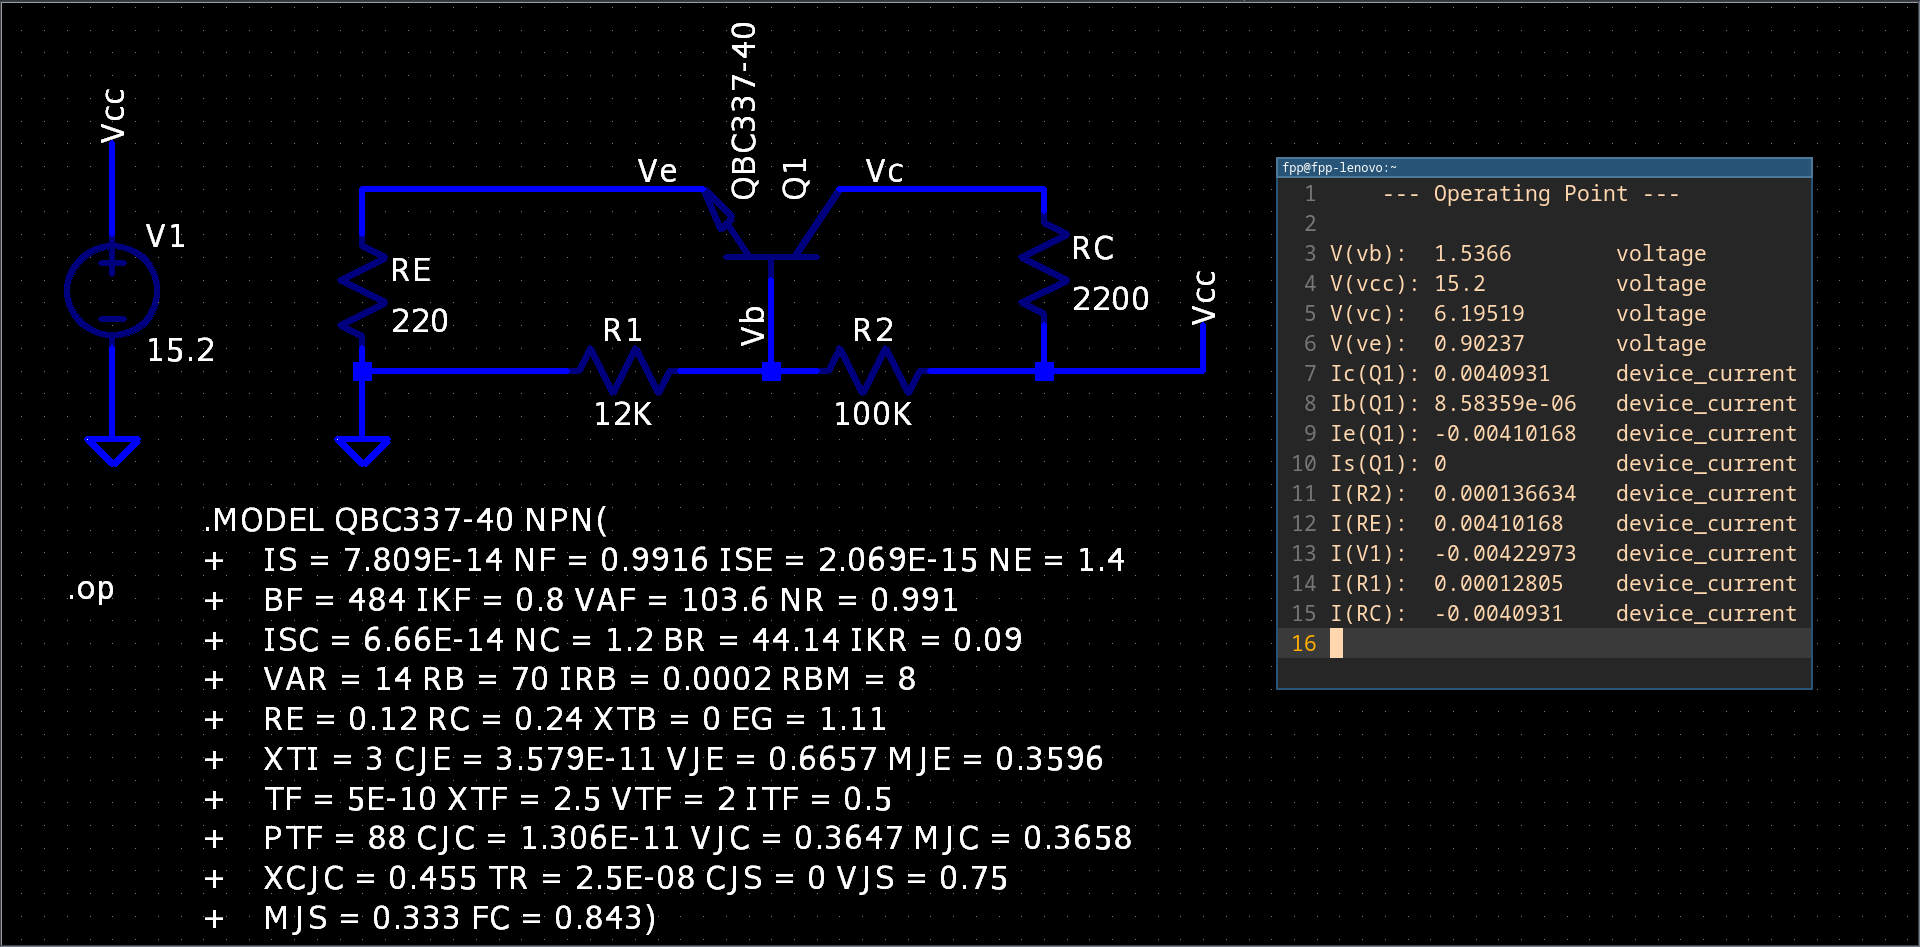
\includegraphics[width=.9\textwidth]{images/sim_normalizada.png}
    \caption{simulación en LTSpice de punto de operación (OP) con resistencias normalizadas.}
  \end{figure}
  \begin{equation*}
    4.07V \leq v_{CBQ} \leq 4.98V \quad \quad 3.7mA \leq i_{CQ} \leq 4.53mA
  \end{equation*}
\end{frame}

\subsection{Pequeña señal}
\begin{frame}[allowframebreaks]{Análisis de pequeña señal}
  \begin{figure}[ht!]
    \begin{minipage}[][\textheight][]{\textwidth}
      \centering
      \resizebox{\textwidth}{!}{
      \begin{tikzpicture}
        % Paths, nodes and wires:
        \draw (3.5, 1.25) to[american resistor, l_={$R_C$}] (3.5, -1.5);
        \draw (-3.5, -1.5) to[american resistor, l={$R_E$}] (-3.5, 1.25);
        \draw (5.5, 1.25) to[american resistor, l_={$R_L$}] (5.5, -1.5);
        \draw (-5.5, 1.25) to[sinusoidal voltage source, l_={$v_i$}] (-5.5, -1.5);
        \draw (-1.5, -1.5) to[american resistor, l={$h_{ib}$}] (-1.5, 1.25);
        \draw (1.5, 1.25) to[american current source, mirror, l_={$h_{fb} \cdot i_e$}] (1.5, -1.5);
        \draw (-5.5, -1.5) -- (7, -1.5);
        \node[ocirc] at (7, 1.25){};
        \node[ocirc] at (7, -1.5){};
        \draw (-5.5, 1.25) -- (-1.5, 1.25);
        \draw (1.5, 1.25) -- (7, 1.25);
        \node[shape=rectangle, draw, line width=0.5pt, dash pattern={on 2pt off 2pt}, minimum width=4.982cm, minimum height=4.482cm] at (-0, 0){};
        \node[ground] at (0, -1.5){};
        \draw[-latex] (-1.25, 0.75) |- (-1.75, 1.5);
        \draw[-latex] (-5.75, 0.75) -| (-5.75, 1.5) -- (-5.25, 1.5);
        \node[shape=rectangle, minimum width=0.715cm, minimum height=0.715cm] at (7, -0.25){} node[anchor=north west, align=left, text width=0.327cm, inner sep=6pt] at (6.625, 0.125){$v_o$};
        \node[shape=rectangle, minimum width=0.715cm, minimum height=0.715cm] at (-5.5, 1.875){} node[anchor=north west, align=left, text width=0.327cm, inner sep=6pt] at (-5.875, 2.25){$i_i$};
        \node[shape=rectangle, minimum width=0.715cm, minimum height=0.715cm] at (-1.5, 1.875){} node[anchor=north west, align=left, text width=0.327cm, inner sep=6pt] at (-1.875, 2.25){$i_e$};
        \draw[-latex] (-4.5, -2) -| (-4.5, -0.5) -- (-4, -0.5);
        \draw[-latex] (4.5, -2) |- (4, -0.5);
        \node[shape=rectangle, minimum width=0.715cm, minimum height=0.715cm] at (-4.5, -2.375){} node[anchor=north west, align=left, text width=0.327cm, inner sep=6pt] at (-4.875, -2){$Z_i$};
        \node[shape=rectangle, minimum width=0.715cm, minimum height=0.715cm] at (4.5, -2.375){} node[anchor=north west, align=left, text width=0.327cm, inner sep=6pt] at (4.125, -2){$Z_o$};
        \draw[-latex] (5.25, 1.5) -| (5.75, 0.75);
        \node[shape=rectangle, minimum width=0.715cm, minimum height=0.715cm] at (5.5, 1.875){} node[anchor=north west, align=left, text width=0.327cm, inner sep=6pt] at (5.125, 2.25){$i_l$};
        \node[shape=rectangle, minimum width=0.715cm, minimum height=0.715cm] at (1.5, 1.875){} node[anchor=north west, align=left, text width=0.327cm, inner sep=6pt] at (1.125, 2.25){$i_c$};
        \draw[-latex] (1.75, 1.5) -| (1.25, 1.5) -- (1.25, 0.75);
        \node[shape=rectangle, minimum width=0.715cm, minimum height=0.715cm] at (7, 0.875){} node[anchor=north west, align=left, text width=0.327cm, inner sep=6pt] at (6.625, 1.25){$+$};
        \node[shape=rectangle, minimum width=0.715cm, minimum height=0.715cm] at (7, -1.125){} node[anchor=north west, align=left, text width=0.327cm, inner sep=6pt] at (6.625, -0.75){$-$};
      \end{tikzpicture}
      }
      \caption{circuito equivalente para CA.}
    \end{minipage}
  \end{figure}

  \begin{figure}[!ht]
    \raggedright
    Podemos calcular las impedancias del amplificador:\\
    \centering
    \begin{minipage}[][\textheight][t]{0.45\textwidth}
      Usando REF ZI HIB:
      \begin{align*}
        h_{ib} &= \frac{25mV}{I_{CQ}}\\[6pt]
        Z_i &= R_E // h_{ib}\\[6pt]
        Z_i &= \frac{220\Omega \cdot \frac{25mV}{4.142mA}}{220\Omega + \frac{25mV}{4.142mA}}\\[6pt]
        Z_i &= 5.87\Omega
      \end{align*}
    \end{minipage}
    \hfill
    \begin{minipage}[][\textheight][t]{0.45\textwidth}
      Usando REF ZO:
      \begin{align*}
        Z_o &\approx R_C\\[6pt]
        Z_o &\approx 2K2\Omega
      \end{align*}
    \end{minipage}
  \end{figure}

  \begin{figure}[!ht]
    \raggedright
    Podemos calcular las ganancias del amplificador:\\
    \centering
    \begin{minipage}[t]{0.45\textwidth}
      Usando REF AI:
      \small
      \begin{align*}
        A_i &= \frac{R_C}{R_C + R_L} \cdot \frac{R_E}{R_E + h_{ib}}\\[6pt]
        A_i &= \frac{2K2\Omega}{2K2\Omega + 2K2\Omega} \cdot \frac{220\Omega}{220\Omega + \frac{25mV}{4.142mA}}\\[6pt]
        A_i &= 0.486
      \end{align*}
    \end{minipage}
    \hfill
    \begin{minipage}[t]{0.45\textwidth}
      Usando REF AV:
      \small
      \begin{align*}
        A_v &= \frac{R_C // R_L}{h_{ib}}\\[6pt]
        A_v &= \frac{\frac{2K2\Omega \cdot 2K2\Omega}{2K2\Omega + 2K2\Omega}}{\frac{25mV}{4.142mA}}\\[6pt]
        A_v &= 182.248
      \end{align*}
    \end{minipage}
  \end{figure}

\end{frame}

\section{Implementacion}
\begin{frame}{Implementacion}

\end{frame}

\begin{frame}{}
  \begin{columns}[c] % [c] centra verticalmente
    \column{0.5\textwidth}
      \centering
      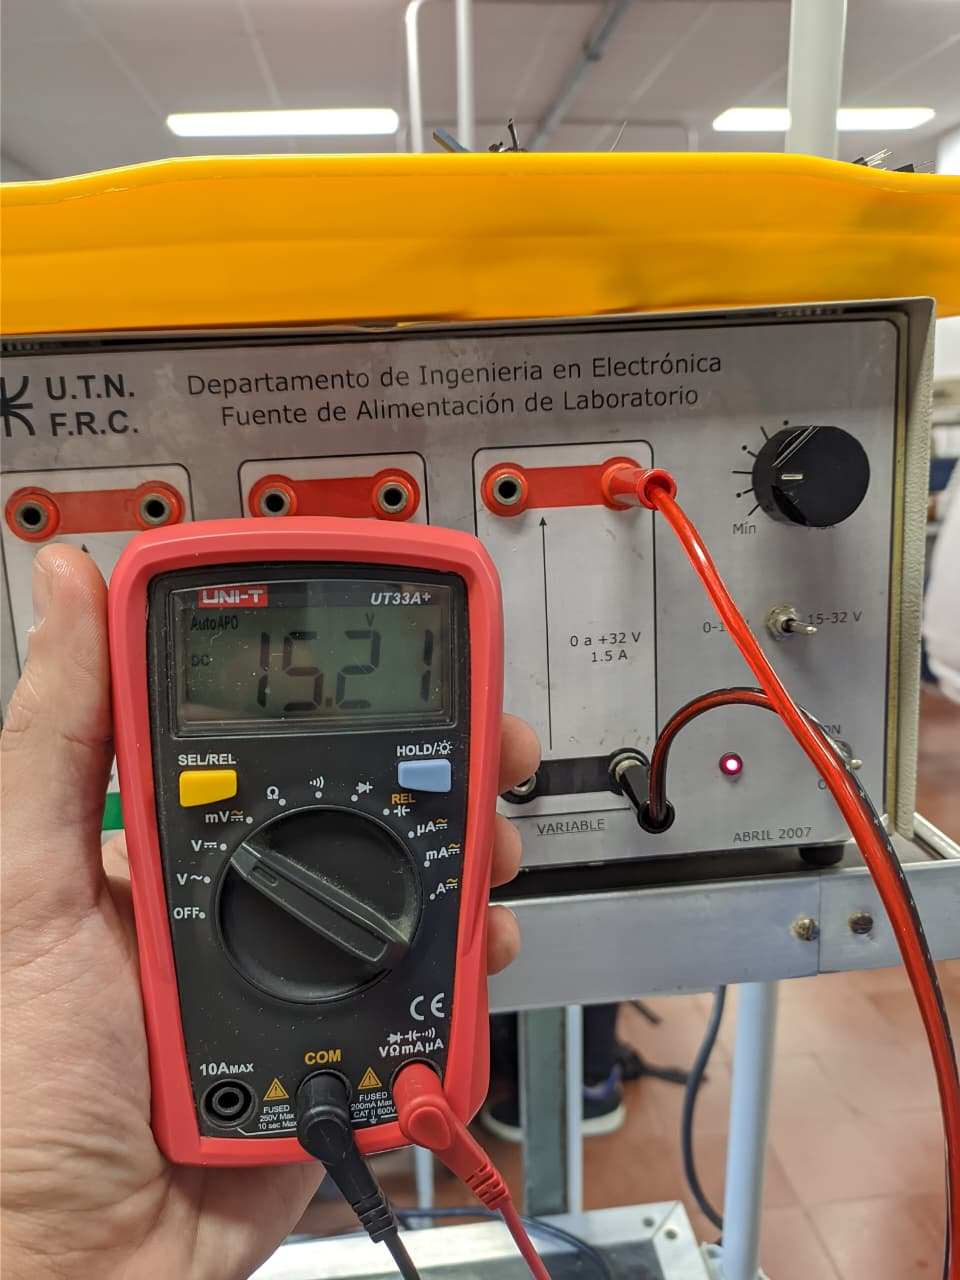
\includegraphics[width=\linewidth]{pictures/VCC.jpeg}

    \column{0.5\textwidth}
      \justifying
        Lo primero que se realiza al energizar el circuito es tomar mediciones de las caidas de tension. como se puede
        apreciar en la foto, esa es la tension de alimentacion VCC. 
      
  \end{columns}
\end{frame}

\begin{frame}{}
  \begin{table}[H]
    \centering
    \caption{Valores medidos y resistencias asociadas}
    \begin{tabular}{lcc}
    \toprule
    \textbf{Parametro} & \textbf{Tensión [V]} & \textbf{Resistencia [\(\Omega\)]} \\
    \midrule
    $V_{CC}$ & $15.21$ & -- \\
    $V_{RC}$ & $9.35$  & $2.18\,k$ \\
    $V_{CB}$ & $4.226$ & -- \\
    $V_{RE}$ & $4.26$  & $217$ \\
    $V_{R1}$ & $1.54$  & $11.96\,k$ \\
    $V_{R2}$ & $13.64$ & $99.7\,k$ \\
    \bottomrule
    \end{tabular}
  \end{table}
\end{frame}


\begin{frame}{}

  \begin{block}{Ecuaciones de referencia}
    \[
      I_{CQ} = \frac{V_{CC} - V_{BB}}{R_C + (R_C \parallel R_L) - \tfrac{R_B}{\beta}}
    \]
    \[
      V_{BB} = V_{CC}\cdot \frac{R_1}{R_1 + R_2}
      \qquad\qquad
      R_B = R_1 \parallel R_2
    \]
  \end{block}

  \begin{block}{Valores calculados}
    \[
      V_{BB} = 1.629 \,\text{V}
      \qquad
      R_B = 10\,678.95 \,\Omega
      \qquad
      I_{CQ} = 4.179 \,\text{mA}
    \]
  \end{block}

\end{frame}


\begin{frame}{}

  \begin{table}[H]
  \centering
  \begin{tabular}{lccc}
    \toprule
    \textbf{Parámetro} & \textbf{Analítico} & \textbf{±10\% del analítico} & \textbf{Calculado} \\
    \midrule
    $I_{CQ}$  & $4.121\,\text{mA}$ & $[3.709\,;\,4.533]\,\text{mA}$ & $4.179\,\text{mA}$ \\
    $V_{CBQ}$ & $4.53\,\text{V}$   & $[4.077\,;\,4.983]\,\text{V}$  & $4.226\,\text{V}$ \\
    \bottomrule
  \end{tabular}
  \end{table}

  \vspace{1em}

  \begin{block}{Observación}
    Los valores calculados se ubican dentro del rango de tolerancia del
    $\pm 10\%$ respecto de los analíticos, lo que confirma la validez del
    procedimiento experimental.
  \end{block}

\end{frame}




\begin{frame}{Parámetros hibridos}
    \begin{columns}[t]
      \column{0.48\textwidth}
      \begin{block}{Impedancia de entrada $Z_i$}
        \[
          i_i = \frac{V_s - V_i}{R_s}
          \qquad
          Z_i = \frac{V_i}{i_i}
        \]
      \end{block}
    
      \begin{block}{Ganancia de tensión $A_v$}
        \[
          A_v = \frac{V_o}{V_i}
        \]
      \end{block}
    
      \column{0.48\textwidth}
      \begin{block}{Ganancia de corriente $A_i$}
        \[
          A_i = \frac{i_o}{i_i}
          = \frac{\tfrac{V_o}{R_L}}{\tfrac{V_s - V_i}{R_s}}
        \]
      \end{block}
    
      \begin{block}{Impedancia de salida $Z_o$}
        \[
          i_o = \frac{V_s - V_o}{R_s}
          \qquad
          Z_o = \frac{V_o}{i_o}
        \]
      \end{block}
    \end{columns}

\end{frame}





\begin{frame}{}
\begin{figure}
  \centering
  \begin{subfigure}[t]{0.65\linewidth}
    \centering
    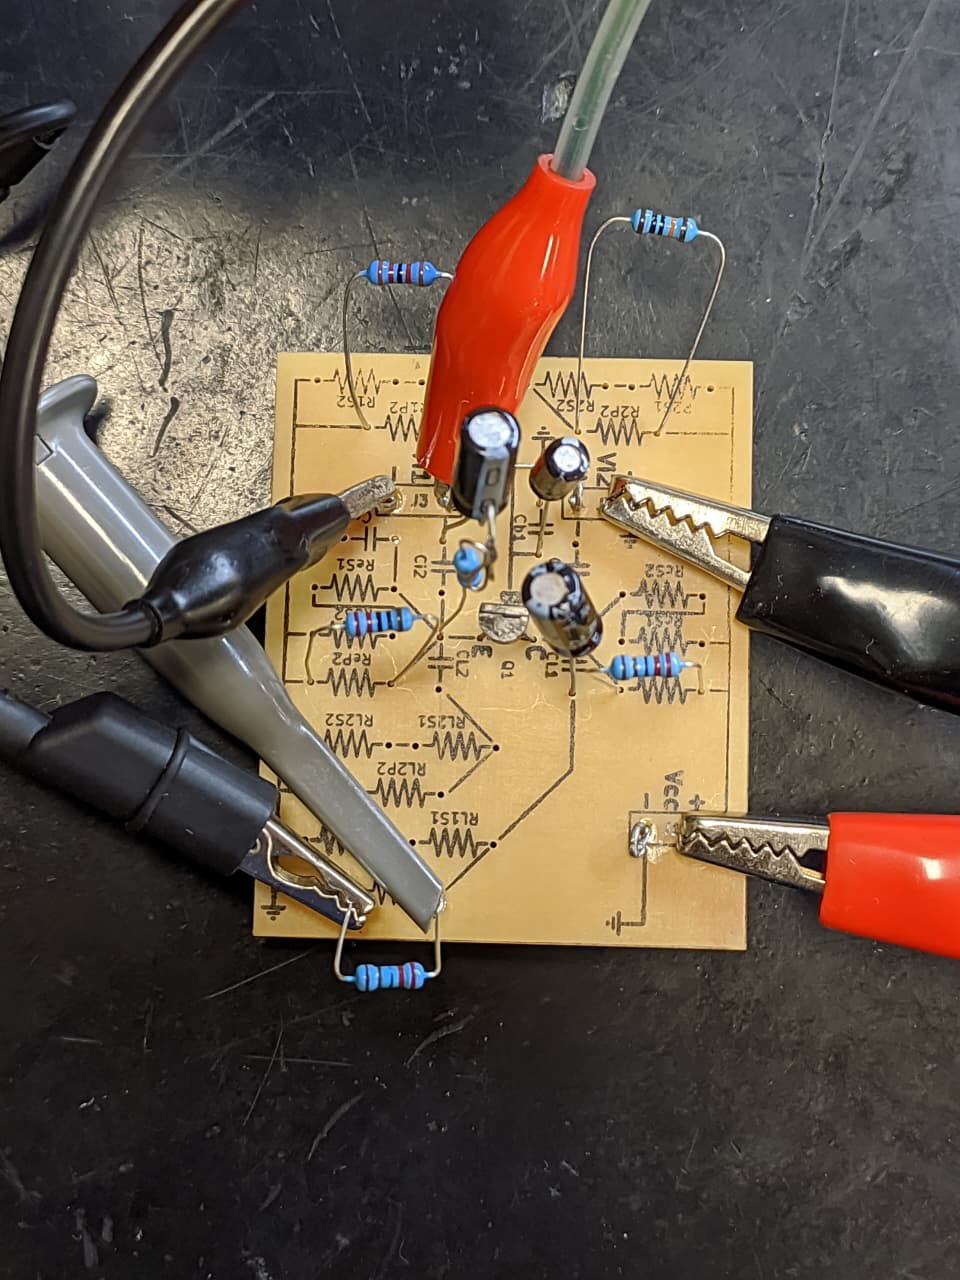
\includegraphics[height=0.65\textheight]{pictures/Placa_Zi.jpeg}
    \caption{Placa montada para medir $Z_i$.}
  \end{subfigure}\hfill
  \begin{subfigure}[t]{0.35\linewidth}
    \centering
    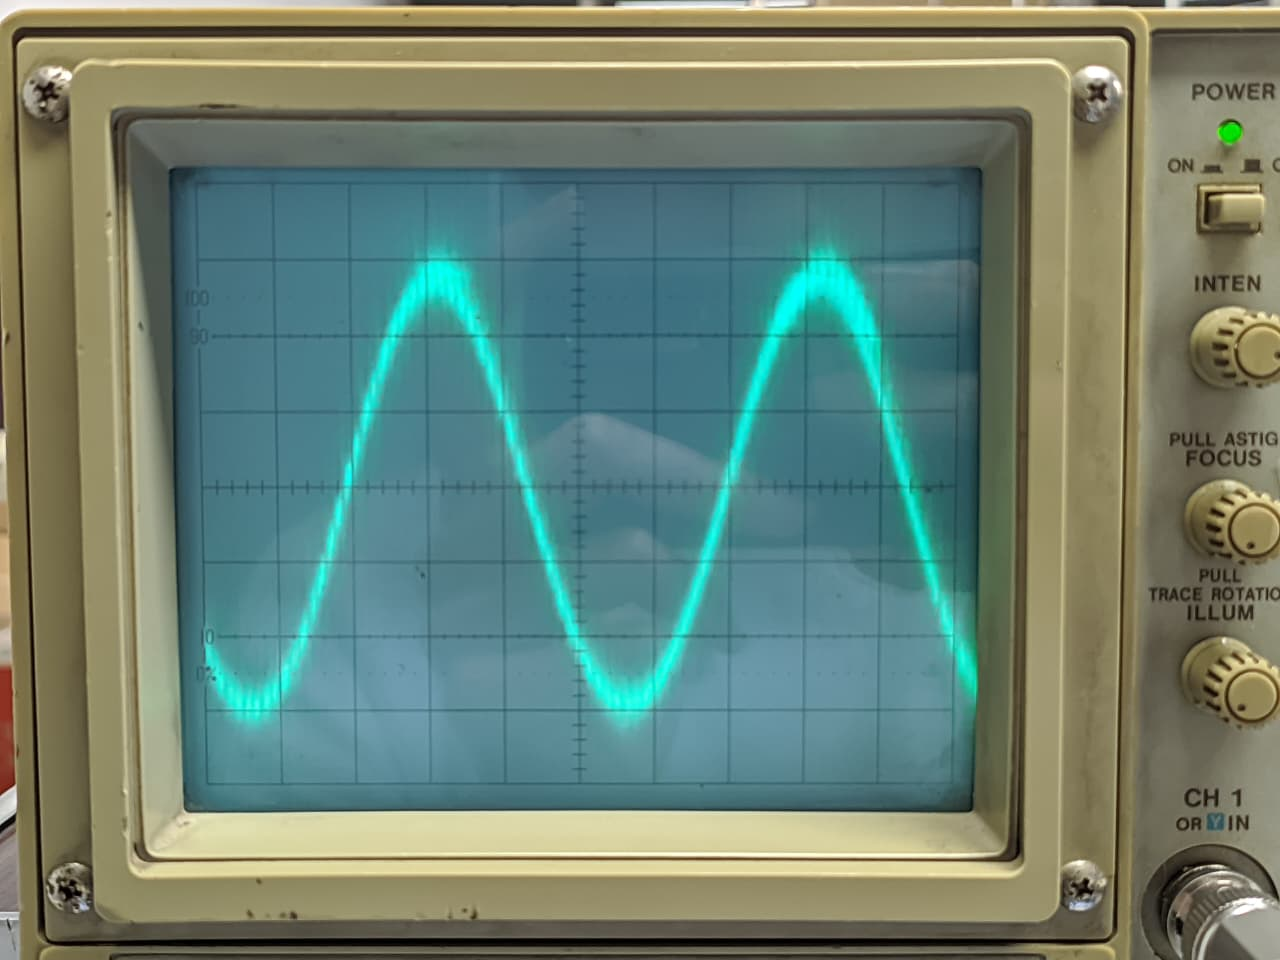
\includegraphics[height=0.35\textheight]{pictures/Medicion Vi.jpeg}
    \caption{$V_i$ en el osciloscopio. Escala: 1\,mV/div, 2\,ms/div.}
  \end{subfigure}
\end{figure}
\end{frame}


\begin{frame}{}

\begin{block}{Ganancia de tensión $A_v$}
\[
A_v = \frac{V_o}{V_i} = \frac{1\,\text{Vpp}}{6\,\text{mVpp}} \approx 166
\]
\end{block}

\begin{block}{Ganancia de corriente $A_i$}
\[
i_i = \frac{V_s - V_i}{R_s} = \frac{6\,\text{mVpp}}{6.8\,\Omega} \approx 0.88\,\text{mA}
\]
\[
i_o = \frac{V_o}{R_L} = \frac{1\,\text{Vpp}}{2.2\,\text{k}\Omega} \approx 0.4545\,\text{mA}
\]
\[
A_i = \frac{i_o}{i_i} = \frac{0.4545}{0.88} \approx 0.516
\]
\end{block}

\begin{block}{Impedancia de entrada $Z_i$}
\[
Z_i = \frac{V_i}{i_i} = \frac{6\,\text{mVpp}}{0.88\,\text{mA}} \approx 6.82\,\Omega
\]
\end{block}

\end{frame}



\begin{frame}{}

\begin{block}{Impedancia de salida $Z_o$}
\[
Z_o = \frac{V_o}{i_o}
\]
\[
i_o = \frac{V_o}{R_L} = \frac{1\,\text{Vpp}}{2.2\,\text{k}\Omega}
\]
\[
Z_o = \frac{1\,\text{Vpp}}{\tfrac{1\,\text{Vpp}}{2.2\,\text{k}\Omega}}
\]
\[
Z_o \approx 2.2\,\text{k}\Omega
\]
\end{block}

\end{frame}

\section{Desafios}
\begin{frame}{Desafios}

\end{frame}


\end{document}
